\documentclass{article}
\usepackage{graphicx}
\usepackage[margin=0.5in]{geometry}
\usepackage{mathtools}
\usepackage{multicol,caption}
\newenvironment{Figure}
  {\par\medskip\noindent\minipage{\linewidth}}
  {\endminipage\par\medskip}

\begin{document}

\title{Ph20 Lab 4: Numerical Solution of Ordinary Differential Equations}
\author{Neil McBlane: 2050386}

\maketitle

\section{Part 1}
\subsection{The Explicit Euler Method}

Figure \ref{fig:s1p1} demonstrates the behaviour of the position and velocity of the simple spring when simulated using the Explicit Euler method. Over time, we see a deviation from the expected constant amplitude.

\begin{Figure}
\centering
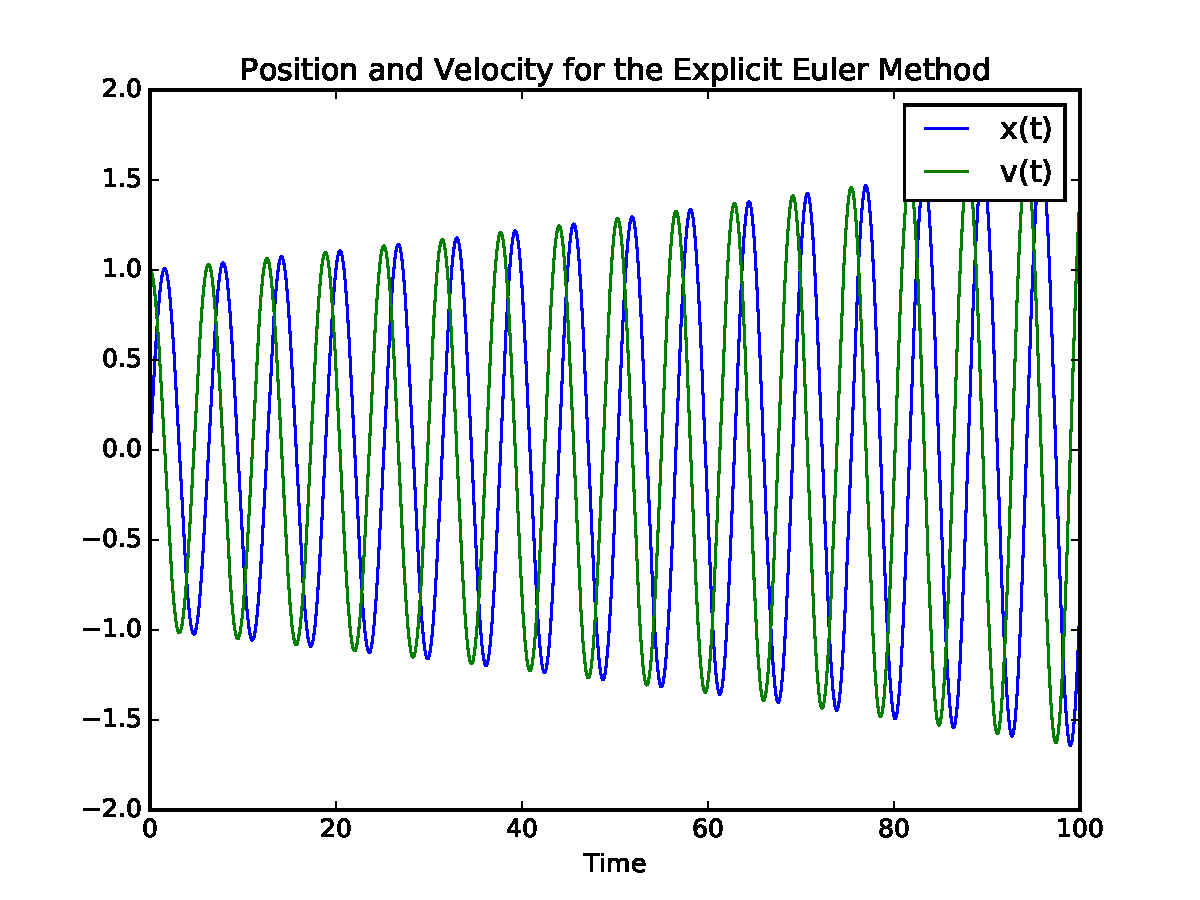
\includegraphics[width=0.7\textwidth]{images/Sec1Plt1.pdf}
\captionof{figure}{Evolution of position and velocity with time for the explicit Euler method, for a timestep of 0.01.}
\label{fig:s1p1}
\end{Figure}

\subsection{The Evolution of Errors}

Figure \ref{fig:s1p2} demonstrates that the difference between the analytic solutions and Explicit Euler solutions for position and velocity reflects the increase in amplitude over time.

\begin{Figure}
\centering
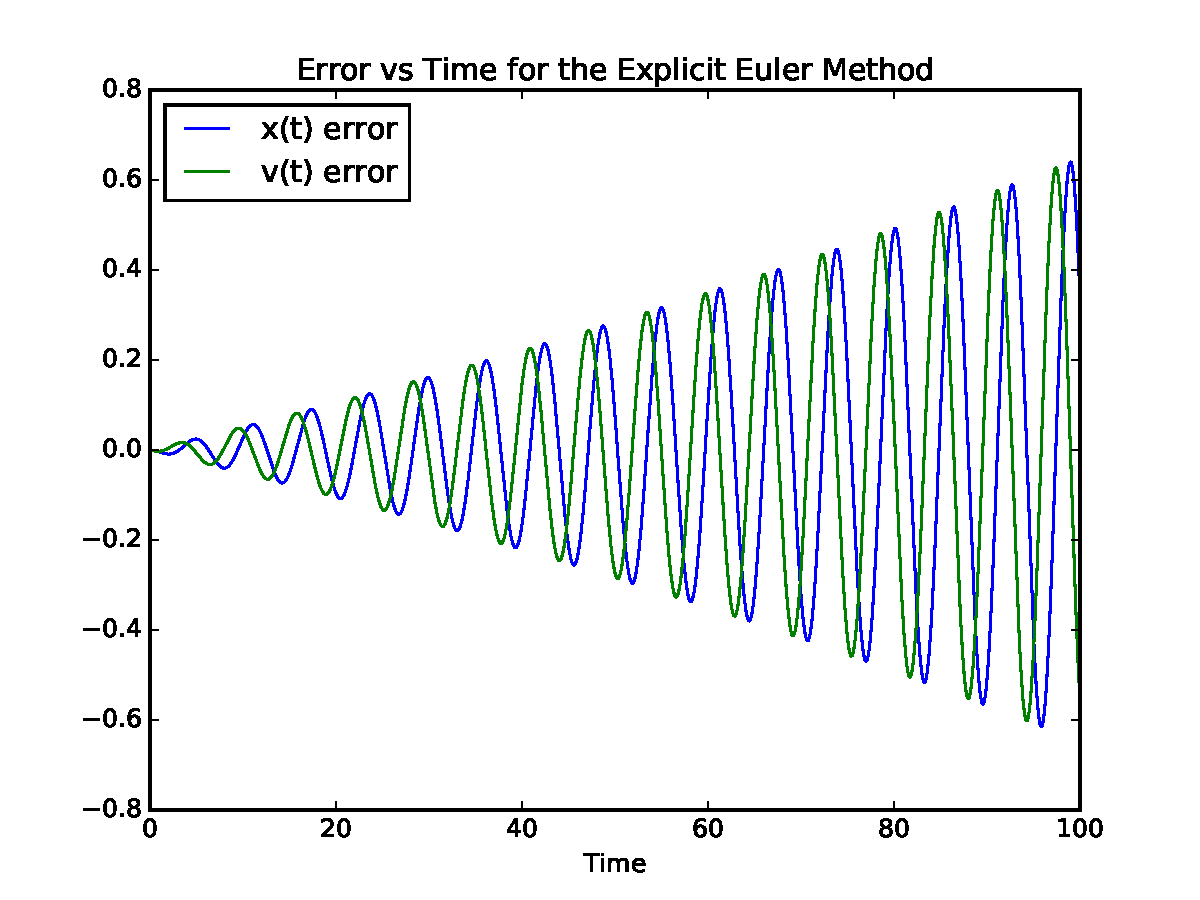
\includegraphics[width=0.7\textwidth]{images/Sec1Plt2.pdf}
\captionof{figure}{Evolution of the error for position and velocity with time for the explicit Euler method, determined by their deviation from the analytically determined solution. Timestep of 0.01 used.}
\label{fig:s1p2}
\end{Figure}


\subsection{Truncation Error}

From figure \ref{fig:s1p3} we see that there is a clear linear relationship between the step size and the truncation error, estimated by taking the maximum position error for a range of simulations taken up to the same final time.

\begin{Figure}
\centering
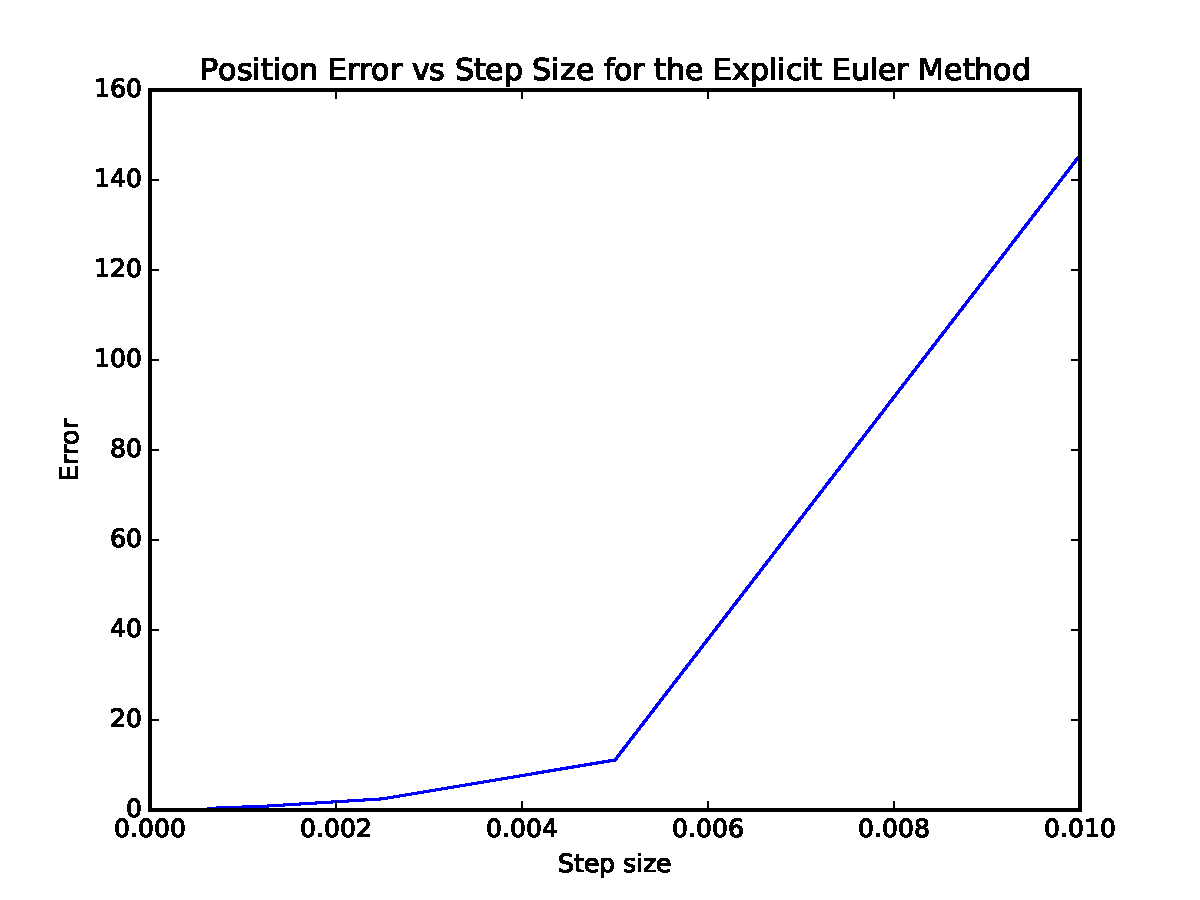
\includegraphics[width=0.7\textwidth]{images/Sec1Plt3.pdf}
\captionof{figure}{The maximum error obtained in a simulation run up to a time of 100 for various timestep sizes.}
\label{fig:s1p3}
\end{Figure}

\subsection{Energy Error}

We expect the energy of the system to be conserved, but figure \ref{fig:s1p4} demonstrates that it increases over time. This reflects the long-term behaviour of position and velocity.

\begin{Figure}
\centering
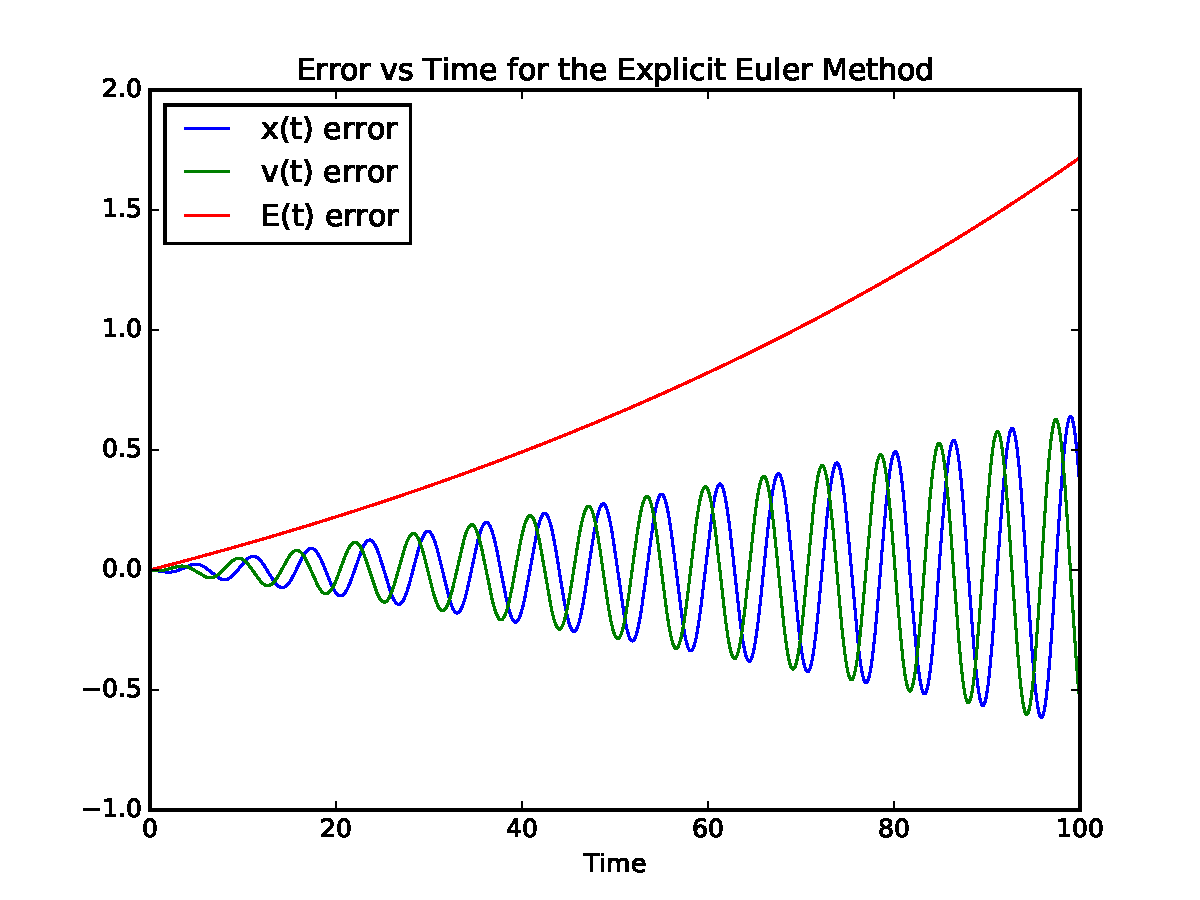
\includegraphics[width=0.7\textwidth]{images/Sec1Plt4.pdf}
\captionof{figure}{The total energy of the system over time, normalised to be at zero initially.}
\label{fig:s1p4}
\end{Figure}

\subsection{The Implicit Euler Method}

Figure \ref{fig:s1p5} shows that the Implicit Euler method demonstrates the same general behaviour as the Explicit method, but on a much slower scale and with a different phase. After 100 seconds, the error in energy is roughly a third that of the Explicit method and is now negative - i.e. the energy is decreasing with time. For position and velocity we see that the sign is also flipped.

\begin{Figure}
\centering
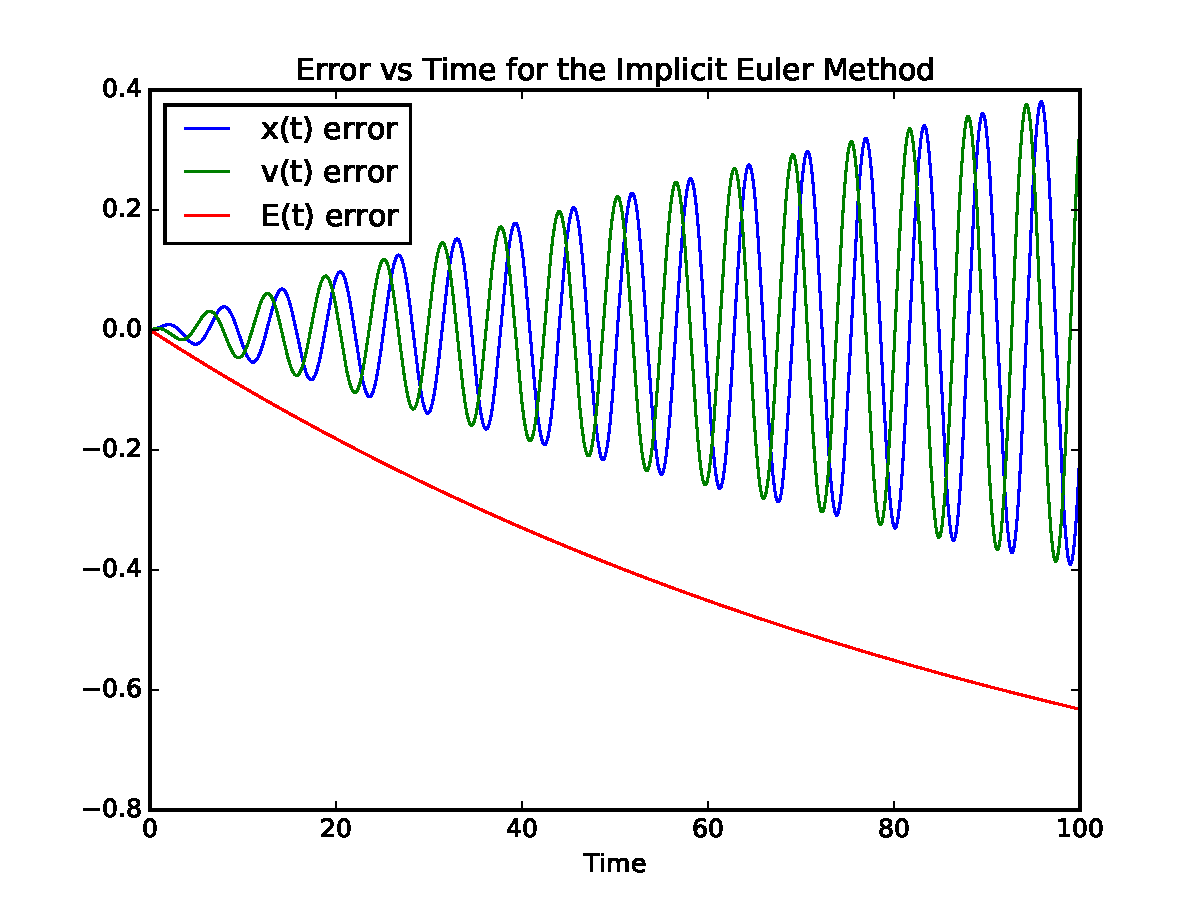
\includegraphics[width=0.7\textwidth]{images/Sec1Plt5.pdf}
\captionof{figure}{The error of the implicit Euler method over time.}
\label{fig:s1p5}
\end{Figure}

\section{Part 2}
\subsection{Implicit and Explicit Euler Phase-Space}

Figure \ref{fig:s2p1} shows that the implicit and explicit Euler methods do not result in closed orbits. Their behaviour reflects the error we see for their evolution in time: the explicit method spirals outwards as its energy increases and the implicit method comes inwards.

\begin{Figure}
\centering
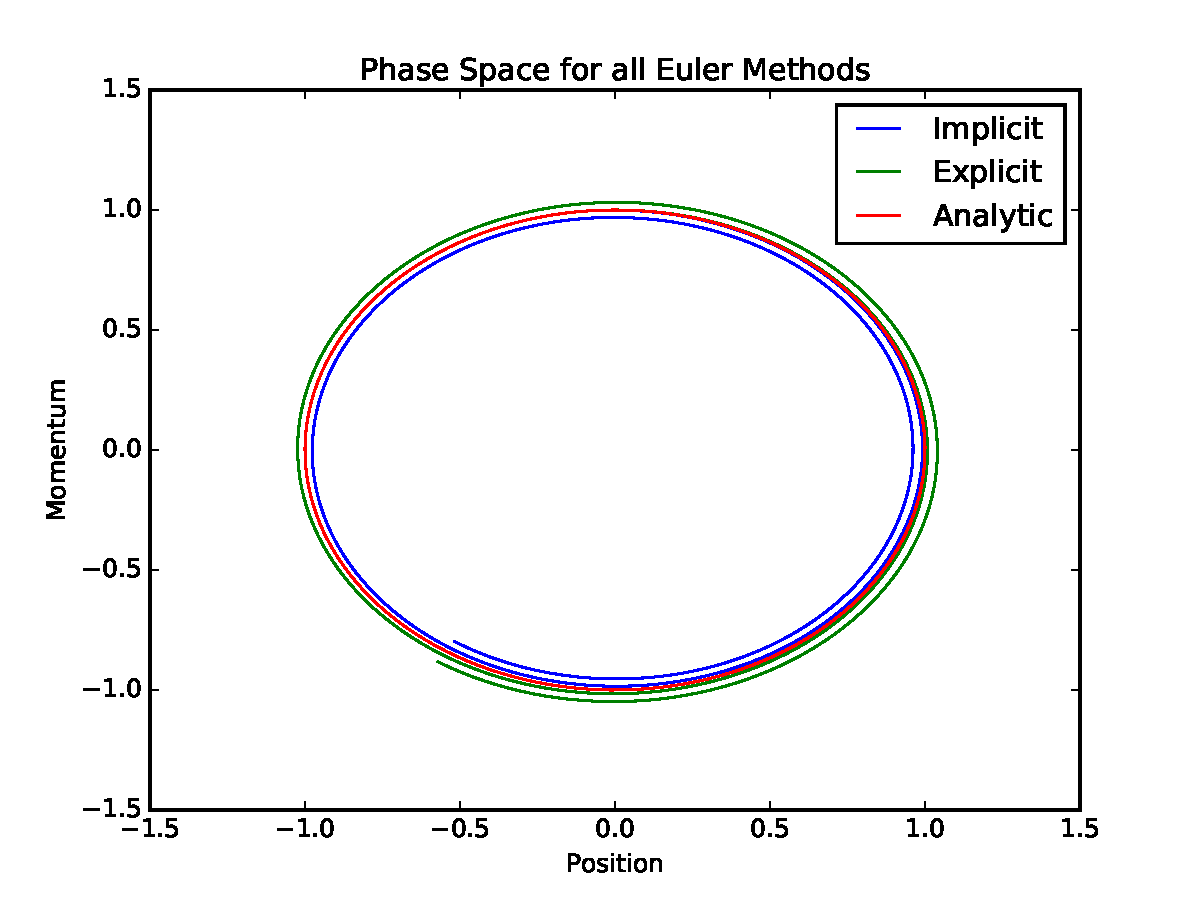
\includegraphics[width=0.7\textwidth]{images/Sec2Plt1.pdf}
\captionof{figure}{The phase space trajectory of the implicit and explicit Euler methods over time, compared to the analytic solution.}
\label{fig:s2p1}
\end{Figure}

\subsection{Symplectic Euler Phase-Space}

For the symplectic method, we still see closed orbits, but they are tilted in phase space compared to the analytic solution; as can be seen in figure \ref{fig:s2p2}.

\begin{Figure}
\centering
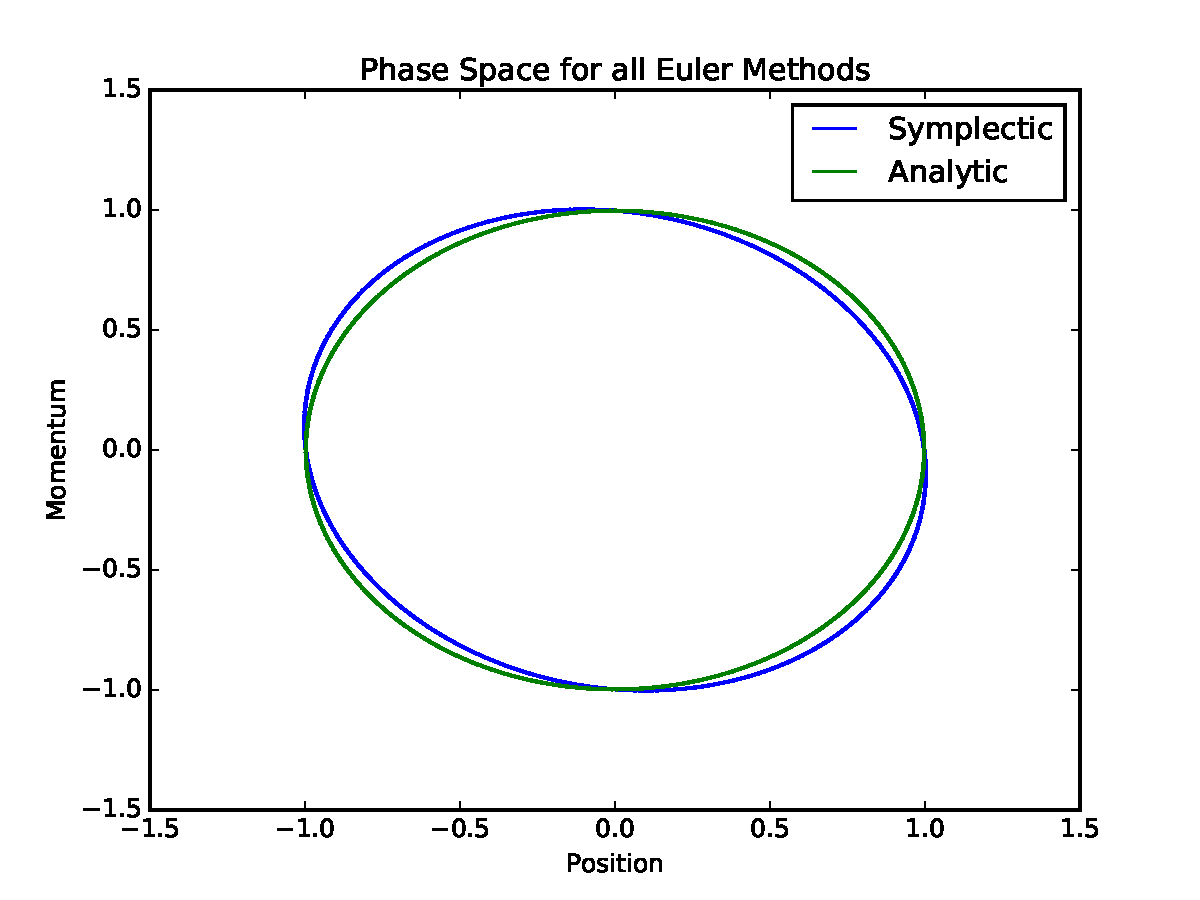
\includegraphics[width=0.7\textwidth]{images/Sec2Plt2.pdf}
\captionof{figure}{The phase space trajectory of the symplectic Euler method over time, compared to the analytic solution.}
\label{fig:s2p2}
\end{Figure}

\subsection{Symplectic Euler Energy}

Figure \ref{fig:s2p3} shows that over time, the error in energy osillates about the constant value we expect. The amplitude of these oscillations is tiny, as we would expect given its accuracy in phase space.

\begin{Figure}
\centering
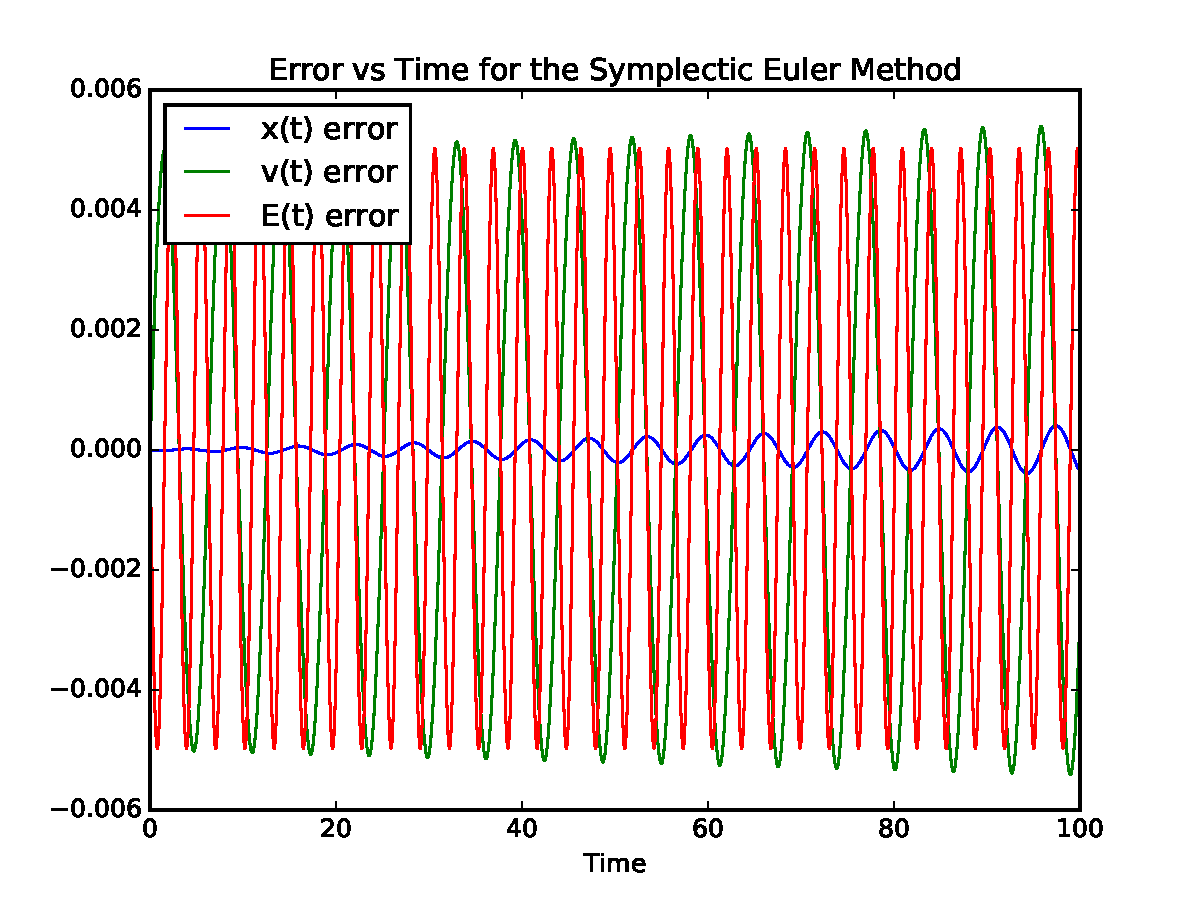
\includegraphics[width=0.7\textwidth]{images/Sec2Plt3.pdf}
\captionof{figure}{The evolution of the errors obtained for the symplectic Euler method with time.}
\label{fig:s2p3}
\end{Figure}

\subsection{Symplectic Euler Phase Error}

From figure \ref{fig:s2p4} we see why there the phase space of the symplectic Euler method is tilted compared to the analytic solution - there is a phase shift between the two, which can be seen after many oscillations.

\begin{Figure}
\centering
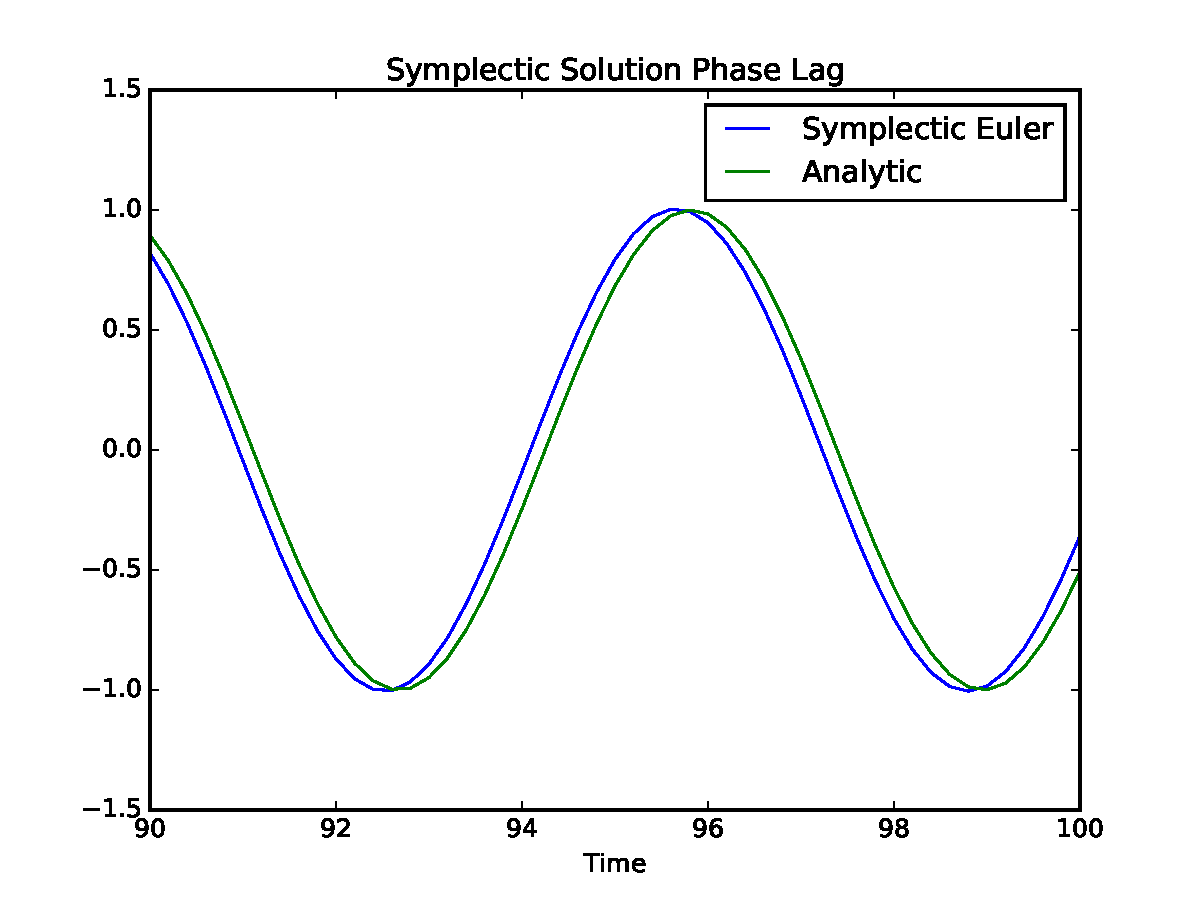
\includegraphics[width=0.7\textwidth]{images/Sec2Plt4.pdf}
\captionof{figure}{The difference in phase between symplectic and analytic solutions. The last few oscillations of a long running simulation are shown as the effect is small.}
\label{fig:s2p4}
\end{Figure}

\end{document}
